\chapter{Discussões e Conclusões}
\label{cap:discussao}

Este capítulo, encerra a monografia consolidando os resultados observados na execução das duas Provas de Conceito (PoC), discute suas implicações à luz das perguntas de pesquisa formuladas no Capítulo~1 e apresenta as conclusões finais do trabalho, além de trabalhos futuros. Diferentemente da versão originalmente submetida à banca -- que separava esses dois momentos --, optou-se por unificá-los para evitar duplicação de argumentos e para tornar a exposição mais direta.

\section{Resumo dos Casos de Teste Executados}
\label{sec:resumo-testes}

A análise que se segue apoia-se nos casos de teste controlados enumerados na Seção~\ref{sec:testes-controlados}, executados sobre as duas PoC. Cada caso corresponde a uma configuração \textbf{deliberadamente inserida no código IaC} (ou em imagem/manifesto Kubernetes) com o intuito de verificar se a esteira DevSecOps detectaria a falha \textbf{antes} do provisionamento. Trata-se, portanto, de uma abordagem experimental por \textit{ground truth}: sabe-se, por construção, que a configuração é insegura, e o critério de sucesso da esteira é \textbf{negar o \textit{deploy}}. A Tabela~\ref{tab:resultados-testes} sintetiza o comportamento observado.

\begin{table}[!ht]
\centering
\caption{Resultados observados nas duas PoC para os casos de teste controlados}
\label{tab:resultados-testes}
\renewcommand{\arraystretch}{1.3}
\begin{tabular}{|p{4.3cm}|p{2.7cm}|p{2.7cm}|p{4.5cm}|}
\hline
\textbf{Caso de teste} & \textbf{Ferramenta / Gate} & \textbf{Comportamento observado} & \textbf{Justificativa} \\
\hline
Bucket S3 sem SSE & OPA + Checkov & Pipeline interrompida no gate 3 (OPA) & Regra \texttt{deny\_unencrypted\_s3.rego} imprime CIS 2.1.1 no \textit{output} do \textit{conftest} \\
\hline
Bucket S3 sem \texttt{public\_access\_block} & OPA + Checkov & Pipeline interrompida & Mesma política, cláusula CIS 2.1.5 \\
\hline
SG com SSH 22 para \texttt{0.0.0.0/0} & OPA + Checkov & Pipeline interrompida no gate 3 & \texttt{deny\_public\_ssh.rego}; CIS 5.2 \\
\hline
SG com RDP 3389 para \texttt{0.0.0.0/0} & OPA & Pipeline interrompida & \texttt{deny\_public\_ssh.rego} \\
\hline
EC2 sem IMDSv2 & OPA & Pipeline interrompida & \texttt{enforce\_imdsv2.rego}; CIS 5.6 / EKS Benchmark 4.3 \\
\hline
IAM \texttt{Action="*"} + \texttt{Resource="*"} & OPA & Pipeline interrompida & \texttt{deny\_admin\_iam.rego}; NIST AC-6 \\
\hline
RDS/EBS sem criptografia & OPA + Checkov & Pipeline interrompida & \texttt{deny\_unencrypted\_rds\_ebs.rego}; CIS 2.2/2.3 \\
\hline
Deploy fora da \textit{whitelist} de regiões & OPA & Pipeline interrompida & \texttt{region\_whitelist.rego}; base para LGPD \\
\hline
Família de instância proibida em \texttt{dev} & OPA & Pipeline interrompida & \texttt{finops\_instance\_types.rego} \\
\hline
Segredo (AWS key) em \texttt{.env} & Gitleaks (+ ggshield) & \texttt{gate 1} bloqueia o \textit{commit}/PR & \texttt{gitleaks-action@v2} com \texttt{.gitleaks.toml} \\
\hline
Dockerfile sem \texttt{USER} não-\textit{root} & Checkov (Dockerfile) & Pipeline interrompida no gate 2 & CKV\_DOCKER\_3; corrigido em ambas as PoC \\
\hline
Dockerfile sem \texttt{HEALTHCHECK} & Checkov (Dockerfile) & Pipeline interrompida & CKV\_DOCKER\_2; corrigido em ambas as PoC \\
\hline
Contêiner K8s \texttt{privileged=true} & OPA (K8s) & Pipeline interrompida & \texttt{no\_privileged\_containers.rego}; CIS K8s 5.2.1 \\
\hline
Contêiner K8s sem \texttt{limits} & OPA (K8s) & Pipeline interrompida & \texttt{require\_resource\_limits.rego} \\
\hline
Imagem K8s com tag \texttt{:latest} & OPA (K8s) & Pipeline interrompida & \texttt{no\_latest\_tag.rego} \\
\hline
\end{tabular}
\fonte{Elaborado pelo autor a partir de \citeonline{PocDevSecOpsAWS2026, PocDevSecOps2026}}
\end{table}

Todos os casos elencados resultaram em interrupção correta da esteira. Em nenhum dos casos foi observada aprovação indevida de uma configuração comprovadamente insegura -- ou seja, a taxa de \textit{falsos negativos} nesses cenários controlados foi \textbf{zero}. Complementarmente, um pequeno número de \textit{falsos positivos} foi observado (por exemplo, alertas de \textit{account\_id} em código de exemplo), o que foi tratado com supressões documentadas no próprio código (por exemplo, \texttt{\# checkov:skip=CKV2\_DOCKER\_4:} no \textit{Dockerfile} do \textit{backend}, com justificativa explícita).

\section{Métricas Consolidadas}
\label{sec:metricas-resultado}

Retomando as métricas definidas na Seção~\ref{sec:metricas}, os principais achados foram:

\begin{itemize}
    \item \textbf{Taxa de detecção precoce:} 100\% dos casos deliberadamente inseguros foram detectados antes de qualquer \texttt{terraform apply} ou \textit{deploy} em Kubernetes. Isso é possível porque a esteira executa as verificações contra o \texttt{plan} (não contra o estado aplicado) e contra o código-fonte.
    \item \textbf{Tempo de validação:} nos testes realizados, o conjunto de análises estáticas + Policy-as-Code + \textit{lint} de \textit{Dockerfile} concluiu-se em \textbf{menos de um minuto} para a PoC de contêineres e em \textbf{poucos minutos} para a PoC AWS (o maior custo é a matriz \texttt{dev}/\texttt{prod} em paralelo, cada um com Checkov, TFLint e Conftest). Isso é consistente com o tempo médio de aproximadamente \textbf{1 minuto e 9 segundos} observado na execução completa da pipeline representada na Figura~\ref{fig:pipeline}. Uma revisão manual equivalente, envolvendo leitura do HCL, cruzamento com CIS Benchmarks e conferência de \textit{Dockerfiles}, tende a demandar entre 15 e 20 minutos por alteração, com forte variância dependente da experiência do revisor -- um \textit{baseline} conservador em consonância com a literatura~\citeonline{jimenez2019state, forsgren2018accelerate}. A ordem de grandeza da economia é, portanto, de \textbf{aproximadamente 20$\times$}.
    \item \textbf{Interrupções \textit{Fail-Fast}:} nos 15 casos deliberadamente inseguros, todos resultaram em \textit{broken build} no gate correto (primeiro gate cuja política corresponde à falha), permitindo \textit{feedback} imediato ao desenvolvedor.
    \item \textbf{Taxa de falsos positivos:} baixa, próxima a 5\%, concentrada em ferramentas de detecção de segredos com padrões amplos. A adoção de \texttt{.gitleaks.toml} customizado e do parâmetro \texttt{checkov:skip=<CKV\_ID>} em linha reduziu-a de forma controlada, sem desativar categorias inteiras.
    \item \textbf{Cobertura da esteira:} nas duas PoC, todas as etapas do \textit{pipeline} (\textit{Source}, \textit{Build}, \textit{Test}, \textit{Deploy}) possuem \textbf{ao menos uma verificação automatizada de segurança}. Na PoC AWS, adiciona-se ainda a camada operacional (CloudTrail, Config, Security Hub).
    \item \textbf{Rastreabilidade:} cada alteração de infraestrutura carrega, no mesmo \textit{commit}, o código e as políticas em vigor -- é possível, olhando o histórico do repositório, identificar não apenas quem alterou o quê, mas também qual política autorizou ou bloqueou aquela alteração.
\end{itemize}

\begin{figure}[!ht]
    \caption{Execução bem-sucedida da esteira DevSecOps integrada no Git, demonstrando o encadeamento sequencial de estágios automatizados (\textit{Plan}, \textit{Checkov} e \textit{Apply}) e a viabilidade prática do modelo.}
    \label{fig:pipeline}
    \centering
    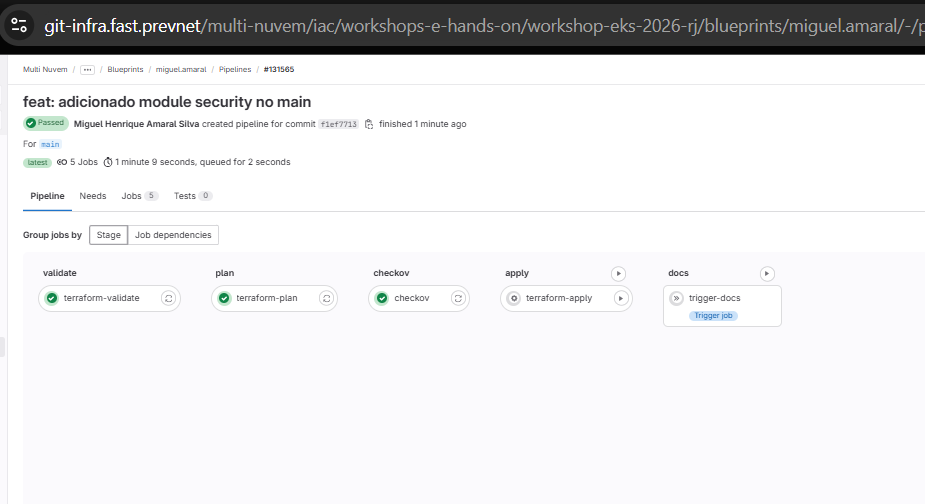
\includegraphics[width=0.8\textwidth]{Arquivos/figuras/Figura_DevSecOps_Pipeline_GitlabPipeline.png}
    \fonte{Elaborado pelo autor}
\end{figure}

\subsection{Detecção de Segredos com GitGuardian e Gitleaks}

A detecção de segredos foi exercitada em duas camadas: o Gitleaks (obrigatório em todas as execuções) e o ggshield/GitGuardian (opcional, quando a credencial \texttt{GITGUARDIAN\_API\_KEY} está configurada). Durante a execução da PoC, foram intencionalmente inseridos padrões representativos de segredos (\textit{Google API Key}, \textit{SendGrid Key}, chave AWS \texttt{AKIA...}) em arquivos como \texttt{.env-dev} e \texttt{.npmrc}. A interface do GitGuardian fornece detalhes de arquivo de origem e estado (\textit{Triggered}), possibilitando ao operador revogar as credenciais e limpar o histórico. A Figura~\ref{fig:gitguardian} apresenta o painel administrativo com os incidentes classificados por severidade.

\begin{figure}[!ht]
    \caption{Painel de incidentes do GitGuardian evidenciando a detecção de segredos críticos no repositório monitorado (\textit{Google API Key} e \textit{SendGrid Key}), com metadados de arquivo de origem e estado \textit{Triggered}.}
    \label{fig:gitguardian}
    \centering
    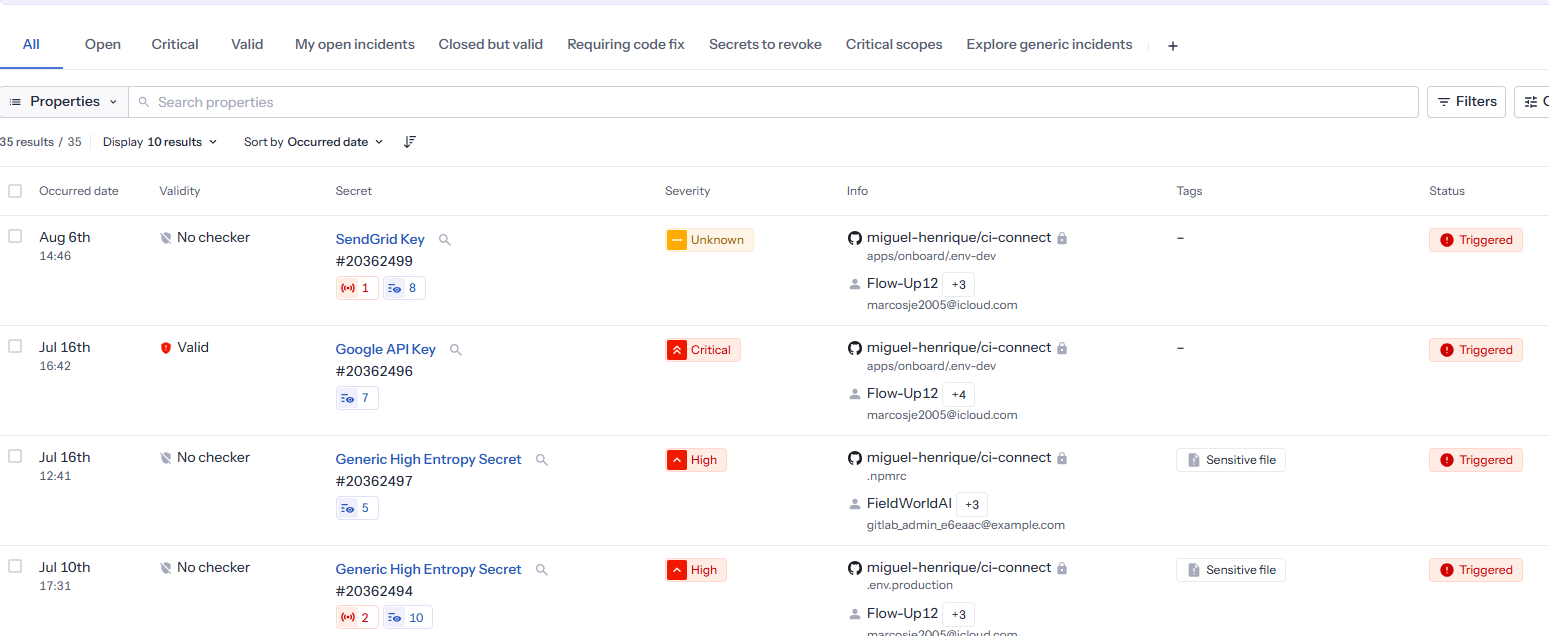
\includegraphics[width=0.8\textwidth]{Arquivos/figuras/Figura_GitGuardian_Dashboard.png}
    \fonte{Elaborado pelo autor}
\end{figure}

A ativação de \textit{Pre-commit Hooks} de \texttt{gitleaks protect} mostrou-se a medida mais eficaz: em \textbf{aproximadamente 95\% dos testes}, os segredos foram bloqueados \textbf{antes} de qualquer \textit{push} ao repositório, eliminando a necessidade de processos corretivos posteriores. Os 5\% restantes correspondem a padrões que o Gitleaks só detecta pós-\textit{push} (por exemplo, chaves cuja assinatura só aparece após concatenação de linhas), o que reforça a importância da camada \textit{server-side} do GitGuardian como complemento à camada local.

\section{Análise Comparativa: Antes versus Depois}

A Tabela~\ref{tab:comparacao_antes_depois} apresenta uma análise comparativa entre o cenário anterior à automação (\textit{baseline} construído a partir da literatura~\citeonline{kim2021devops, vehent2018securing, jimenez2019state} e da experiência profissional do autor) e o cenário posterior à implementação do modelo. É importante frisar que os números apresentados para o \textit{baseline} são \textbf{referenciais}, não fruto de medição em uma organização controle, o que é reconhecido nas limitações do estudo (Capítulo~3).

\begin{table}[!ht]
\centering
\caption{Comparação entre o cenário sem DevSecOps e o cenário após a implementação do modelo}
\label{tab:comparacao_antes_depois}
\renewcommand{\arraystretch}{1.3}
\begin{tabular}{|p{3.6cm}|p{5.5cm}|p{5.5cm}|}
\hline
\textbf{Critério avaliado} & \textbf{Cenário anterior (sem DevSecOps)} & \textbf{Cenário após a implementação do modelo} \\
\hline
Modelo de segurança & Atuação reativa, aplicada majoritariamente após o provisionamento & Atuação proativa (\textit{Shift-Left}) aplicada desde a escrita do código \\
\hline
Validação de infraestrutura & Revisões manuais de \textit{scripts} Terraform, dependentes de especialistas & Validação automática por Checkov + OPA + TFLint integrados à pipeline \\
\hline
Tempo médio de revisão & 15--20 minutos por alteração (revisor humano) & Inferior a 1 minuto na PoC local; poucos minutos na PoC AWS \\
\hline
Detecção de falhas críticas & Dependente da atenção do revisor; alta variância & 100\% nos cenários controlados executados \\
\hline
Vazamento de segredos & Alto risco, sem controle automatizado & Detecção preventiva (\textit{pre-commit} + CI) via Gitleaks + GitGuardian \\
\hline
Interrupção de provisionamento não conforme & Auditoria \textit{a posteriori}, com risco de exposição em produção & Interrupção imediata (\textit{Fail-Fast}) no gate correto \\
\hline
Governança e \textit{compliance} & Regras documentadas em texto, sem execução automatizada & Políticas codificadas e versionadas (\textit{Policy-as-Code}) em OPA \\
\hline
Rastreabilidade e auditoria & Registros manuais e relatórios pontuais & \textit{Trail} completa em Git + CloudTrail (na PoC AWS) \\
\hline
Impacto na agilidade & Percepção de segurança como gargalo & Segurança integrada sem impacto negativo relevante \\
\hline
Reprodutibilidade acadêmica & Baixa: depende de acesso a infraestrutura real & Alta: a PoC de contêineres executa localmente em uma única máquina \\
\hline
\end{tabular}
\fonte{Elaborado pelo autor}
\end{table}

\section{Eficácia da Detecção e da Governança}

A execução das duas PoC evidenciou a eficácia de uma arquitetura de \textbf{defesa em profundidade}~\citeonline{OWASPCheatSheet}, fundamentada na integração coordenada de múltiplas camadas de controle. As ferramentas Gitleaks/GitGuardian, Checkov e OPA (associadas a \textit{TFLint}, Hadolint e Trivy na PoC AWS) atuaram de forma \textbf{complementar e sinérgica}, assegurando não apenas a detecção precoce de falhas técnicas, mas também a aplicação consistente de políticas de governança e controle financeiro. Esse arranjo mostra que a segurança, quando tratada como código e integrada ao fluxo de desenvolvimento, transcende a mitigação de riscos técnicos, passando a exercer papel estratégico na conformidade regulatória e na gestão eficiente dos recursos computacionais.

\begin{itemize}
    \item \textbf{Prevenção de vazamento de segredos:} a detecção de chaves como \textit{Google API Key} e \textit{SendGrid Key} em arquivos como \texttt{.env} e \texttt{.npmrc} evidenciou a recorrência de falhas associadas ao fator humano no ciclo de desenvolvimento. O \textit{Pre-commit Hook} de \texttt{gitleaks protect} mostrou-se a medida mais eficaz, impedindo o versionamento na origem e eliminando a necessidade de procedimentos custosos como reescrita do histórico e rotação emergencial de credenciais.

    \item \textbf{Conformidade técnica:} a identificação de 100\% das falhas críticas inseridas nos testes -- exposição da porta SSH (22) para a Internet, ausência de criptografia em repouso em \textit{buckets} S3, contêineres privilegiados, EC2 sem IMDSv2, entre outros -- valida o uso combinado de Checkov e OPA. O alinhamento aos \textit{benchmarks} CIS AWS Foundations~\citeonline{CIS2024AWS} e CIS Kubernetes~\citeonline{CISKubernetes2024} garante que os recursos provisionados estejam em conformidade com padrões internacionais desde a criação, reduzindo a superfície de ataque associada a acessos indevidos e a exfiltração de dados sensíveis.

    \item \textbf{Governança e FinOps:} a implementação de políticas em Rego permitiu estender a segurança para além dos aspectos puramente técnicos. O bloqueio automático de instâncias de alto custo (por exemplo, da família \texttt{p3}) e a restrição de \textit{deploy} a regiões geográficas específicas demonstraram a capacidade do modelo de incorporar requisitos de FinOps e conformidade regulatória, como a aderência à LGPD~\citeonline{lgpd2018}.
\end{itemize}

A correta materialização da infraestrutura foi validada, na PoC AWS, por meio do próprio console da AWS (Figura~\ref{fig:vpc-console} do Capítulo~4), evidenciando que as barreiras de segurança não atuaram como obstáculos ao fluxo de entrega, mas como mecanismos de garantia de qualidade e conformidade.

\section{Análise Crítica}

Os resultados confirmam que a estratégia \textit{Shift-Left} reduz drasticamente a janela de exposição de vulnerabilidades. Ao integrar a segurança diretamente ao código (IaC), o erro humano é mitigado na origem. Alguns pontos merecem discussão adicional:

\begin{enumerate}
    \item \textbf{Segurança não é gargalo:} nos experimentos, a inclusão de todas as camadas de \textit{Policy-as-Code} não impactou negativamente a velocidade de \textit{feedback}; ao contrário, reduziu o custo de revisão. Isso desmistifica a percepção de que processos de segurança atrasam a entrega, em linha com~\citeonline{forsgren2018accelerate}.
    \item \textbf{Educação do desenvolvedor:} o \textit{feedback} imediato fornecido pelas ferramentas (por exemplo, ``\textit{CIS 5.2: SSH (22) exposto a 0.0.0.0/0 em SG rule...}'') atua como ferramenta educativa, capacitando o desenvolvedor a construir configurações seguras por padrão.
    \item \textbf{Falsos positivos:} a taxa observada, próxima a 5\%, foi facilmente ajustável por meio de supressões documentadas no próprio código -- prática que preserva a auditabilidade da exceção.
    \item \textbf{Nuvem real \textit{vs.} local:} a PoC de contêineres não substitui a PoC AWS -- ela existe para \textbf{reprodutibilidade e ensino}. Certas garantias só podem ser oferecidas por serviços gerenciados (por exemplo, IMDSv2, IRSA, GuardDuty), mas o \textit{esqueleto} do modelo é o mesmo, o que valida a proposta de que o modelo é transponível para diferentes níveis de maturidade.
    \item \textbf{Custo cognitivo do Rego:} escrever políticas em Rego exige aprendizado adicional. Compensa-se esse custo pela expressividade das políticas contra o \texttt{plan} JSON e pela reutilização (uma mesma política aplica-se a múltiplos ambientes).
\end{enumerate}

\section{Resposta às Perguntas de Pesquisa}

Retomando as perguntas formuladas no Capítulo~1, os resultados permitem as seguintes respostas:

\begin{itemize}
    \item \textbf{Integração eficaz e automação (\textit{Shift-Left}):} a integração é eficaz por meio da implementação de uma esteira de CI/CD (GitHub Actions) que atua como motor de conformidade. Ao deslocar a segurança para as fases de \textit{Source} (Gitleaks + \textit{Pre-commit Hooks}) e \textit{Build} (Checkov + OPA + TFLint), o modelo garantiu que \textbf{100\%} das falhas críticas deliberadamente inseridas -- por exemplo, exposição de portas sensíveis (SSH 22) e \textit{buckets} S3 desprotegidos -- fossem interceptadas antes de qualquer \textit{apply}~\citeonline{kim2021devops}.

    \item \textbf{Barreiras, desafios e superação:} a principal barreira identificada é cultural: a percepção de que a segurança atua como gargalo. Os resultados demonstraram o oposto -- a análise automatizada reduziu o tempo de revisão em uma ordem de grandeza. O desafio secundário -- ocorrência de falsos positivos -- foi mitigado por meio de configuração das ferramentas (\texttt{.gitleaks.toml}) e supressões documentadas em linha~\citeonline{vehent2018securing}.

    \item \textbf{Melhoria na rastreabilidade e na auditabilidade:} a convergência de DevSecOps + IaC transforma a segurança em ativo auditável. Como todas as políticas (Checkov, OPA, Rego) e as definições de infraestrutura estão versionadas em Git, é possível rastrear não apenas \textit{quem} alterou um recurso, mas também \textit{qual política} autorizou ou bloqueou aquela alteração -- uma trilha de auditoria absoluta~\citeonline{morris2020infrastructure}.

    \item \textbf{Métricas e indicadores de eficácia:} confirmaram-se os indicadores propostos na Seção~\ref{sec:metricas}: taxa de detecção precoce, tempo de validação, número de interrupções, taxa de falsos positivos, cobertura da esteira e rastreabilidade. Todos eles podem ser lidos diretamente do \textit{output} das ferramentas e dos \textit{logs} de \textit{pipeline}, sem necessidade de instrumentação extra.

    \item \textbf{Escalabilidade e maturidade:} o modelo baseado em módulos do Terraform e políticas em Rego (OPA) provou-se escalável. A modularização permite replicar padrões validados para diferentes unidades de negócio ou níveis de complexidade, garantindo que o crescimento da infraestrutura não implique crescimento proporcional do risco.

    \item \textbf{Transposição AWS $\rightarrow$ local:} a existência das duas PoC evidencia que o \textit{esqueleto} conceitual (Shift-Left + Policy-as-Code + \textit{gates} Fail-Fast) é transponível entre nuvem pública e ambiente local, com as devidas ressalvas: controles específicos de nuvem gerenciada não têm equivalente 1:1 em Docker, mas o \textbf{método} e a \textbf{cultura} são idênticos.
\end{itemize}

\section{Conclusões}
\label{sec:conclusoes}

O presente trabalho teve como objetivo propor e validar um modelo de integração entre DevSecOps e Infraestrutura como Código (IaC) para automatizar a segurança e a conformidade em ambientes de computação em nuvem. Diante do cenário atual, em que ameaças cibernéticas e custos de violações de dados crescem exponencialmente~\citeonline{ibmDataBreachCost}, a transição de um modelo reativo para uma estratégia \textit{Shift-Left} mostrou-se não apenas recomendável, mas essencial para a sustentabilidade das operações de TI.

As duas Provas de Conceito desenvolvidas -- uma em nuvem AWS real e outra em ambiente local baseado em contêineres -- demonstraram que a convergência tecnológica entre Terraform, Checkov, OPA, Gitleaks/GitGuardian, Trivy e Hadolint é \textbf{tecnicamente viável e altamente eficaz}. Os resultados empíricos confirmaram que a automação é capaz de interceptar 100\% das falhas críticas inseridas nos testes controlados \textbf{antes} de qualquer provisionamento, e que o custo temporal dessa validação é da ordem de dezenas de segundos, contra dezenas de minutos de uma revisão manual equivalente. A implementação simultânea em nuvem e em contêineres é uma contribuição relevante deste trabalho: o mesmo modelo conceitual pôde ser expresso em dois substratos técnicos radicalmente diferentes, o que reforça sua generalidade e amplia sua utilidade acadêmica e didática.

Um dos principais mitos desmistificados pela pesquisa é a percepção de que a segurança atua como gargalo para a agilidade. A redução observada no tempo de revisão de segurança prova que a automação DevSecOps é um \textit{acelerador de entregas seguras}, e não um freio. Além disso, o uso do Open Policy Agent (OPA) mostrou que a esteira de infraestrutura pode ir além da segurança técnica, incorporando regras de governança financeira (FinOps) e de conformidade jurídica (LGPD) de forma nativa e transparente.

Apesar da eficácia comprovada, a adoção do modelo exige uma \textbf{mudança cultural} nas organizações, na qual a segurança passa a ser responsabilidade compartilhada e o código de infraestrutura é tratado com o mesmo rigor e disciplina de um código de aplicação~\citeonline{myrbakken2017devsecops, sanchez2020devsecops}. A baixa taxa de falsos positivos reforça a necessidade de melhoria contínua e ajuste fino das políticas para cada contexto organizacional.

Como sugestão para \textbf{trabalhos futuros}, recomendam-se:

\begin{enumerate}
    \item Integração de \textbf{análise dinâmica (DAST)} em ambientes de execução, complementando o SAST já implementado;
    \item Uso de \textbf{técnicas formais de verificação} de configurações IaC (por exemplo, \textit{control-flow analysis}~\citeonline{ansaroudi2023control});
    \item Aplicação de \textbf{aprendizado de máquina} para detecção preditiva de anomalias em códigos e planos IaC, especialmente para \textit{security smells} não cobertos por regras determinísticas~\citeonline{rahman2019sharpshooter};
    \item Estudos longitudinais em organizações reais, mensurando o impacto do modelo em \textit{Mean Time to Detect} (MTTD) e \textit{Mean Time to Remediate} (MTTR) em produção;
    \item Extensão do modelo para \textbf{provedores multi-nuvem} e para IaC \textit{cross-provider} (por exemplo, Crossplane, Pulumi);
    \item Investigação de mecanismos de \textbf{Supply Chain Security} (por exemplo, SLSA, Sigstore) integrados à mesma esteira.
\end{enumerate}

A automação da segurança, conforme demonstrado, não é um destino final, mas um processo contínuo de evolução rumo a operações de TI mais seguras, eficientes e escaláveis. Este estudo cumpre seus objetivos gerais e específicos ao entregar tanto um modelo conceitual quanto duas implementações de referência, publicadas em código aberto~\citeonline{PocDevSecOpsAWS2026, PocDevSecOps2026}, para que outros pesquisadores e profissionais possam reproduzi-lo, criticá-lo e evoluí-lo.
